%%%%%%%%%%%%%%%%%%%%%%%%%%%%%%%%%%%%%%%%%%%%%%%%%
% Relatório Final - Projeto de Pesquisa
% Métodos de Otimização
% Baltz & Machado
% Capítulo 1
%%%%%%%%%%%%%%%%%%%%%%%%%%%%%%%%%%%%%%%%%%%%%%%%%


\chapter{\Large{Métodos Matemáticos de Otimização}}\label{chp:1}


\section{{Sobre o Conceito de Otimização}}

\hspace{0.8cm}
Diz-se otimização, o processo que tem como objetivo encontrar condições que
minimizam ou maximizam algo (seja energia, tempo, dinheiro, etc). Sendo este,
muitas vezes um trabalho árduo, custoso.

Dessa maneira, na matemática, tal processo é amplamente utilizado quando
busca-se valores em um conjunto \( A \) (que pode ter restrições), com o
objetivo de encontrar uma solução ótima (a melhor resposta para o problema),
aplicando os valores de \( A \) em uma função objetivo predefinida.


\begin{definition}[Conceito de otimização]
    Dada uma função  \( f : A \subseteq \mathbb{R} \rightarrow \mathbb{R}. \)
    Onde \( A \) é um conjunto  conexo da reta real.
    Dizemos que \( x^* \in A \) é um ótimo para a função \( f \) se alguma das
    condições abaixo forem satisfeitas:
    \begin{enumerate}
        \item Se \( f(x^*) \leq f(x) \), para todo \( x \in A \);
        \item Se \( f(x^*) \geq f(x) \), para todo \( x \in A \).
    \end{enumerate}

    E diremos que \( x^* \) é uma solução ótima para o problema de otimização da
    função \( f(x) \) restrito ao conjunto \( A \).

\end{definition}

Podemos então esclarecer a significância das condições satisfeitas por um ótimo.
Diremos que \( x^* \) é um \textit{máximo de \( f(x) \)} quando a condição
\textit{1} for satisfeita e \( x^* \) será dito um \textit{mínimo de \( f(x) \)}
quando a condição \textit{2} for satisfeita. Além disso, o conceito de conexo
inserido no contexto da definição revela a intrínsica necessidade de controle
sobre os valores de entrada. Um exemplo de conjunto conexo seria um intervalo
na reta.

Agora vamos tentar entender como esse processo pode ser custoso. A princípio
temos o fato de que uma função \( f(x) \) pode assumir seus pontos máximos e
mínimos que podem ser locais ou globais. Devemos compreender os pontos máximos
(mínimos) como \textit{ótimos locais} como sendo aqueles que não
são os maiores (menores) valores para a maximização (minimização). E como
\textit{ótimos globais} aqueles que são os maiores (menores)
valores para a maximização (minimização).

O custo a que nos referimos é devido a incerteza de classificar, em geral, pontos que
satisfaçam essas tais características. Como se pode perceber na Figura
\ref{grafico_local_global_pontosCriticos}.

\begin{figure}[h]
    \centering
    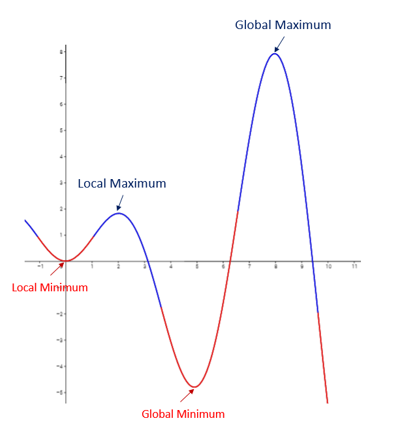
\includegraphics[width=0.43\textwidth]{src/grafico_local_global_pontosCriticos.png}
    \captionsetup{justification=centering}
    \caption{
      Exemplo de pontos críticos locais e globais indicados no gráfico de uma função.\\
      \tiny Essa imagem foi coletada de \url{https://www.onlinemathlearning.com}.
    }
    \label{grafico_local_global_pontosCriticos}
\end{figure}

Como na grande maioria dos casos não é possível conhecer antecipadamente todo o
conjunto dos pontos imagem, a busca pelo ótimo pode resultar em ótimos locais.
A depender do problema, tais resultados chegam a ser satisfatórios. No entanto,
quando o objetivo é estritamente encontrar os máximos ou mínimos globais, o
trabalho necessário acaba sendo mais custoso, pelo fato
de que há a incerteza da existência de tais pontos na grande maioria dos
problemas.

Ademais, o conjunto $A$, o qual contém os valores aplicáveis na função, pode
ser definido através de restrições, fazendo com que o gráfico da função não
seja contínuo.

\section{{Otimização de Funções à Uma Variável Real}}\label{otim_uma_var}

\hspace{0.8cm}
Evidentemente, as funções possuem as variáveis dependentes (que representam o
objeto da otimização) e as variáveis independentes (que suas grandezas podem
ser selecionadas), podemos denotar que, para a equação
\begin{equation}
    y = f(x),
\end{equation}
quando buscamos otimizá-la, temos como objetivo encontrar valores, \(x\), que
quando aplicados à \(f(x)\), temos o mínimo ou máximo valor \textit{y} (seja
ele local, ou preferencialmente, global).

Partindo dessa perspectiva, acaba surgindo a necessidade de utilizar algum
recurso para encontrar os pontos críticos. E nesse sentindo, pode-se utilizar
a técnica de \textbf{derivação}, que oferece o recurso de identificar tais
pontos.


Podemos observar um fator interessante; por exemplo,
quando a função está num ponto máximo, existem duas possibilidades, a primeira,
a função para de crescer e, em seguida, torna-se indefinida; e a
segunda possibilidade, quando a função para de crescer e começa a decrescer.
Com isso, é importante ressaltar que por definição, quando a derivada (taxa de
variação) em um ponto é positiva, a função cresce, e quando é negativa a função
decresce. Conclui-se que, quando a taxa de variação é zero, a função ou para de
crescer ou de decrescer, o que configura um ponto de máximo ou de mínimo. Mas
também, é quando pode ocorrer o que denominamos ponto de sela (é um
comportamento errático da função, que precisa de uma análise mais refinada). Ou
em última instância, quando a função é constante.

Com o uso da derivada, podemos pensar num método de otimização bastante simples,
considerando \(f(x)\) a função que queremos otimizar e \(f'(x)\) sua função
derivada, podemos dizer que o conjunto $O$, abaixo definido, possui todos os
ótimos locais e globais de \(f(x)\):

\begin{equation}
    O := \{f(x) | f'(x) = 0\}.
    \label{equacao_conjunto_o}
\end{equation}


Portanto, aplicando um filtro em $O$ para obter o máximo e mínimo do conjunto,
acabamos por obter o máximo e mínimo de \(f(x)\):


\begin{equation}
    max(f(x)) = max(O),
\end{equation}

\begin{equation}
    min(f(x)) = min(O).
\end{equation}


Então podemos perceber três problemas:

\begin{itemize}
  \item Determinar como encontrar os pontos onde a derivada se anule, isto é,
    os pontos críticos;
  \item Determinar se temos de fato todos os pontos;
  \item Classificação dos pontos críticos, que nos revela quais são os máximos e
  os mínimos, e, ademais, da sua relevância quanto a serem locais ou globais.
\end{itemize}


\begin{definition}[Pontos Críticos]
    Considerando $f(x)$ como a função objetivo, os pontos críticos dessa função
    são definidos como pontos onde a função é diferenciável e que a derivada é
    anulada. Desse modo, dizemos que o ponto $x$ é crítico quando:

    \begin{equation}
        f'(x) = 0; x \in A.
    \end{equation}

\end{definition}


Consideraremos, por agora, apenas o problema de encontrar os pontos críticos.

A taxa de variação de uma função, \(y=f(x)\), em relação a \(x\), é dada pela
relação \(\Delta y / \Delta x\). Sendo o cálculo da derivada
demonstrado pela Figura \ref{derivada_padrao}, o que nos leva ao fato de que
os pontos críticos provém do conjunto solução da equação \(f'(x) = 0\), como
definido na equação \ref{equacao_conjunto_o}. Além disso, caso a função esteja
definida num intervalo fechado, temos pelo Teorema do Valor Absoluto, a
garantia que ela atingirá o valor dos seus pontos extremos, ou seja, seus
valores de máximo e mínimo serão atingidos naquele intervalo. O que culmina
nossa busca pelos pontos críticos.

\begin{figure}[h]
    \centering
    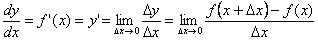
\includegraphics[width=0.45\textwidth]{src/derivada_padrao.jpg}
    \captionsetup{justification=centering}
    \caption{
        Derivada: taxa de variação \(dy/dx\).\\
        \tiny Essa imagem foi coletada de \url{https://brasilescola.uol.com.br}.
    }
    \label{derivada_padrao}
\end{figure}

Partindo desse pressuposto, é nítido que a derivada de uma função é também uma
função. Portanto, fica evidente que uma função pode ser derivada
mais de uma vez, sendo essas derivadas, denominadas de ``primeira derivada'',
``segunda derivada'' e por ai em diante. De modo que, a segunda derivada é
a derivada da primeira derivada. Concluindo-se que dada a função
\(f(x)\), sua primeira derivada é \(df/dx = p(x)\), e sua segunda derivada
\(dp/dx = s(x)\).

Agora vamos tratar da classificação dos pontos críticos.

É sabido que a primeira derivada representa a taxa de variação instantânea de
um ponto na curva, e, que, a segunda derivada proporciona informações
complementares, como por exemplo, se é um ponto de máximo, mínimo ou inflexão,
de modo que, ela determina a concavidade da curva naquele ponto. Como pode ser
visto na Figura \ref{relacao_primeira_segunda_derivada}. E, de modo construtivo,
devemos ressaltar que é importante o estudo do gráfico das derivadas de uma
função, pois é necessariamente através do uso da interpretação do comportamento
da primeira derivada e/ou da segunda derivada, que obtemos a classificação dos
pontos críticos seguindo os critérios que são apontados na Figura \ref{relacao_primeira_segunda_derivada}.

\begin{figure}[h]
    \centering
    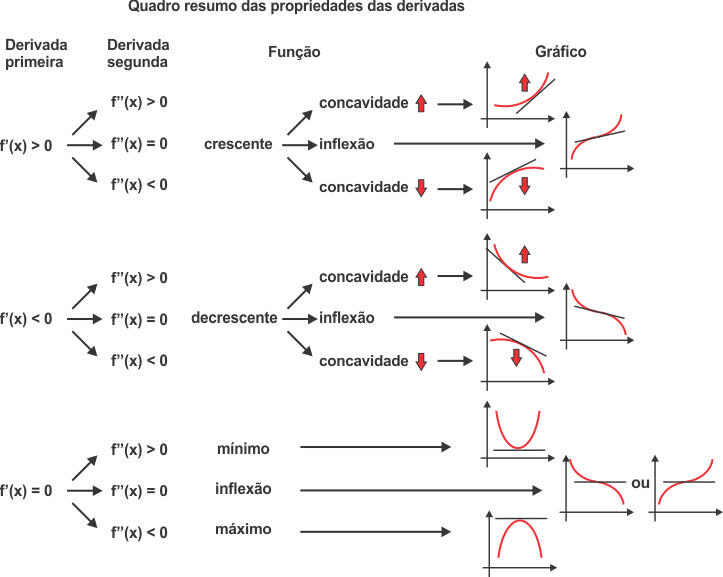
\includegraphics[width=0.65\textwidth]{src/relacao_primeira_segunda_derivada.jpg}
    \captionsetup{justification=centering}
    \caption{
        Propriedades e relação da primeira e segunda derivada.\\
        \tiny Essa imagem foi coletada de \url{https://www.alfaconnection.pro.br}.
    }
    \label{relacao_primeira_segunda_derivada}
\end{figure}


\section{{Programando o Método}}

\hspace{0.8cm}


A própria definição da derivada já nos oferece uma visão simples de como
ela pode ser implementada num programa de computador. Mas, com alguns nuances
que devem ser levados em consideração, segue a tal implementação:


\begin{lstlisting}[]

pub fn derive1x1_v1<F>(f: &F, x: f64) -> f64
where
    F: Fn(f64) -> f64,
{
    (f(x + h) - f(x)) / h
}


\end{lstlisting}


Essa implementação é ingênua no que diz respeito a precisão da operação. O
uso, depende da aplicação, caso se queira prezar por velocidade de cálculo e
muito pouco sobre precisão, então provavelmente, essa solução seja boa o
suficiente. O problema com a precisão desta implementação é que não se é
levado em consideração o aspecto infinitesimal da variação (\(\Delta x\) na
Figura \ref{derivada_padrao}, ou a variável \textit{h} na implementação
em Rust), já que é por este aspecto que definimos a derivada. Não temos como ter
uma variável com tal propriedade num programa de computador. Como consequência,
\(f(x + h) - f(x)\) já é calculada de forma falha, entregando uma variação
diferente da que seria quando se tem uma variável infinitesimal. O que de fato
é entregue, é a variação um pouco mais à frente do ponto esperado.

A partir daí podemos reformular, considerando esse deslocamento, redefinindo
da seguinte forma:


\begin{equation}
    f'(x) = \frac{f(x + h) - f(x - h)}{2h}.
\end{equation}

Que é equivalente à:

\begin{equation}
    f'(x) = \frac{f(x + h) - f(x - h)}{(x + h) - (x - h)}.
\end{equation}


Usaremos essa segunda formulação por motivos de custo de multiplicação de de
números reais se comparado a somas e subtrações, além da possível perda de
precisão. Assim, conseguimos compensar o tal deslocamento numa nova função
insignificantemente mais custosa, e mais precisa. Como vemos no código a seguir:

\begin{lstlisting}[]

pub fn derive1x1_v2<F>(f: &F, x: f64) -> f64
where
    F: Fn(f64) -> f64,
{
    let x1 = x - h;
    let x2 = x + h;

    let y1 = f(x1);
    let y2 = f(x2);
    return (y2 - y1) / (x2 - x1);
}


\end{lstlisting}



\section{{Otimização de Funções à Várias Variáveis}}

\hspace{0.8cm}
Quando encontramos a necessidade de trabalhar com mais dimensões, que na
otimização se traduz no fato de a função trabalhar com mais parâmetros a serem
otimizados, e a saída da função não necessariamente ser um valor real,
temos a necessidade de trabalharmos com funções que tanto na entrada como na
saída, se utilizam de vetores que podem conter uma ou mais variáveis. Portanto,
é necessário estender as ferramentas criadas para funções à uma variável, as
quais apresentamos na seção \ref{otim_uma_var}, para funções de várias
variáveis. Que formalmente se apresenta da seguinte forma:

% TODO: Colocar nesse modelo as demais Definições já escritas
\begin{definition}[Funções Reais à Várias Variáveis]
    Consideramos uma função real à $n$ variáveis uma função $g$ definida em um
    subconjunto $D$ de \(\mathbb{R}^n\) com imagem em \(\mathbb{R}^m\) para
    $n$, $m$ \(\in \mathbb{N^*}\). Isto é,

    \begin{equation}
            g: D \subseteq \mathbb{R}^n \rightarrow \mathbb{R}^m.
    \end{equation}

    Consideraremos $g(x)$ = $y$, com o $x=(x_1, x_2, ..., x_n)$
    e $y=(y_1, y_2, ..., y_n)$.

\end{definition}



Antes de seguirmos, podemos ajustar um pouco a função para facilitar o processo
de otimização. Como a imagem da função pode ser um vetor com mais de uma
entrada, torna-se um pouco mais difícil decidir qual a melhor imagem. Sendo
assim, pode ser muito conveniente reduzir o vetor em uma única medida. Uma das
formas de fazer isto é pela norma euclidiana. Portanto, podemos definir uma
nova função para ser otimizada a partir da original, da seguinte forma:


\begin{equation}
        f(x) = ||g(x)|| = ||y||.\\
\end{equation}
        Onde a norma utilizada é dada pela expressão:
\begin{equation}
        ||y|| = \sqrt{ y_1^2 + y_2^2 + \hdots + y_m^2}.
\end{equation}

Já tendo em mãos um bom formato para as funções que desejamos otimizar, agora
precisamos definir como se dá o processo de derivação para tais funções.

% TODO: Provar essa proposição
Para isto, basta estender o processo que já temos para funções à uma variável,
de forma que ainda seja simples calcular. Vamos começar imaginando a seguinte
situação: temos uma função que define um plano, cuja entrada é um vetor de
duas variáveis e que tem como saída um valor real, de acordo com a definição
dada acima. Para que possamos usar o processo definido para funções à uma
variável, devemos considerar apenas uma secção da superfície dessa função.
Assumindo que todos os elementos do vetor de entrada da função são sempre
constantes, exceto o elemento referente à dimensão que queremos derivar, então
obtemos a derivada na dimensão escolhida. Se repetirmos o processo para a outra
variável do vetor de entrada, teremos então dois vetores que representam as
derivadas em cada direção das seções de corte.

Os argumentos que fizemos nos mostram como replicar o processo de obtenção do
que é a derivada pontual de uma função, agora à duas variáveis. A seguir
apresentamos a definição de derivada parcial:

\begin{definition}[Derivadas Parciais]

    Vale salientar que o cálculo do limite para funçãos à duas variáveis
    difenrencia-se no caso de funçãoes reais à uma variável. Quando calculamos
    o limite de funções reais à duas variáveis, devemos atentar para o fato
    de que aqui fazemos uso da aproximação por curvas arbritárias, o que
    dinamiza a complexidade do cálculo de tal limite, fazendo deste um elemento
    muito mais sofisticado do que o que tiamos no caso à uma variável.

    Considerando uma função real $f$ definida em um subconjunto $D$ $\subseteq$ \(\mathbb{R}^2\). Definimos como as derivadas parciais de $f(x, y)$ os seguintes limites, quando existirem:

    \begin{equation}
        \begin{array}{ccc}
            &   \displaystyle {\dfp{f}{x}(x, y) = \lim\limits_{h \to 0} \frac{f(x+h, y) - f(x, y)}{h},}\\
            &\\
            &   \displaystyle {\dfp{f}{y}(x, y) = \lim\limits_{h \to 0} \frac{f(x,y+h) - f(x,y)}{h}.}\\
        \end{array}
    \end{equation}

\end{definition}

Consideramos que a função é diferenciável no ponto \( (x_0, y_0) \) quando as
derivadas paciais existirem para tal ponto. Vale ressaltar que ambos os limites
devem concomitantemente existir. E chamamos essas derivadas como derivada
parcial em x e em y, respectivamente.

Equivalentemente a como fizemos para funções à uma variável podemos agora
definir o que seria a derivada de uma função à duas variáveis.

\begin{definition}[Diferencial de $f(x, y)$]
    Considerando uma função de $f(x, y)$ diferenciável, definimos o diferencial
    de $f(x, y)$ como sendo:

    \begin{equation}
        Df = \dfp{f}{x} \cdot dx + \dfp{f}{y} \cdot dy.
    \end{equation}

\end{definition}

Observe que uma condição \textit{sine qua non} para que a função seja
diferenciável é que exista o diferencial. Pois isto implica na existência das
derivadas paciais que são coeficientes da combinação linear que define o
diferencial.

Estamos agora em posição de definir um instrumento de grande valor para a
análise de otimização de funções reais a duas variáveis, que denominaremos de
gradiente de $f(x, y)$.

\begin{definition}[Gradiente de $f(x, y)$]

    Considerando uma função de $f(x, y)$ diferenciável e o diferencial como
    definido acima, o vetor gradiente de $f(x, y)$ é aquele que satisfaz:

    \begin{equation}
        Df \cdot v = \left\langle \nabla f, v \right\rangle.
    \end{equation}

    Vemos que o $\nabla f(x, y)$ = $\left(\dfp{f}{x}, \dfp{f}{y}\right)$.


\end{definition}

    %TODO: Mostrar uma proposição (mostrar que o gradiente é a direção em que a função cesce ou decresce mais rapidamente [usar cos talvez])
    \begin{proposition}
        TODO: $\nabla$ é a direção de otimalidade de função
    \end{proposition}

% TODO: Definir curvas de nível
% TODO: Definir matriz Hessiana (Falar da H nula)
% TODO: Classificar pontos críticos a partir da Hessiana
% TODO: Ver teorema espectral
% Pontos criticos = entradas do gradiente nulas; jacobiana nula=pontos criticos
% Dica: uso do polinomio de taylor para duas variaveis

Podemos considerar esse mesmo processo para função cujos vetores de entrada são
maiores, de modo que o gradiente será representado por uma maior quantidade de
derivadas parciais. Com isso, o processo de otimização é similar ao que foi
visto na seção \ref{otim_uma_var}, sofrendo apenas uma adaptação quanto a
quantidade de variáveis que precisam ser modificadas. Ademais, o dado processo
ainda tem como objetivo encontrar valores para essas variáveis de entrada, que
cada vez mais minimizam o vetor gradiente, resultando assim numa aproximação
para um ponto crítico daquela função.

E desse modo, é interessante ressaltar que a norma do vetor gradiente é reduzida
cada vez mais em relação a distância do ponto crítico. Ou seja, quanto mais
próximo do ponto crítico, menor será a norma do vetor.

Com a definição de gradiente posta, podemos ainda definir o que seria o
semelhante ao gradiente para as funções mais gerais, como
\( g: \mathbb{R}^n \rightarrow \mathbb{R}^m \),
e obtendo uma noção mais precisa sobre as ferramentas que temos.


\begin{definition}[Matriz Jacobiana]
    Seja \( g(x) \) uma função vetorial definida em um subconjunto
    \( D \subseteq \mathbb{R}^n \), \( x \in D \),
    e sua imagem o \( \mathbb{R}^m \), podemos escrever
    \( g(x) = (g_1(x), g_2(x), ..., g_m(x)) \). Sabemos que \( g_i(x) \) é
    uma função de \( \mathbb{R}^n \rightarrow \mathbb{R}, i = 1, 2, ... m \),
    considerando o gradiente como uma matriz linha, definimos a Matriz
    Jacobiana de \(g\) em \(x\) como:

    \begin{equation}
        J(g(x)) = \begin{bmatrix}
                    \nabla g_1(x) \\
                    \nabla g_2(x) \\
                    \vdots \\
                    \nabla g_n(x)
                  \end{bmatrix}.
    \end{equation}

    Ou ainda, se expandirmos o gradiente, temos a Matriz Jacobiana \( m \times n \)
    completa com as seguintes entradas:

    \begin{equation}
        J(g(x)) = \begin{bmatrix}
                    \dfp{g_1}{x_1} & \dfp{g_1}{x_2} & \hdots & \dfp{g_1}{x_n}\\
                    \\
                    \dfp{g_2}{x_1} & \dfp{g_2}{x_2} & \hdots & \dfp{g_2}{x_n}\\
                    \vdots & \vdots & \ddots & \vdots \\
                    \dfp{g_m}{x_1} & \dfp{g_m}{x_2} & \hdots & \dfp{g_m}{x_n}\\
                  \end{bmatrix}.
    \end{equation}


\end{definition}

%TODO: falar da jacobiana nula


%
